\chapter{Espaces vectoriels normés}
En première année, nous avons étudié les réels, les suites de réels et les fonctions numériques. Un outil important est la valeur absolue. Elle permet d'évaluer la distance entre deux réels $x$ et $y$: $|x-y|$
\section{Distance}
\begin{definition}
    Soit $E$ un ensemble, une distance $d$ est une fonction de $E\times E$ dans $[0,+\infty[$ vérifiant :
    \begin{enumerate}
        \item $\forall x,y\in E \quad d(x,y)=0 \Leftrightarrow x=y$
        \item $\forall x,y\in E \quad d(x,y)=d(y,x)$
        \item $\forall x,y,z \in E \quad d(x,y)\leq d(x,z)+d(z,y)$
    \end{enumerate}
\end{definition}
\begin{exemple}
Sur $\mathbb{R}$, l'application $d(x,y)=|x-y|$ est une distance. Sur $E$ un ensemble non vide, l'application (distance discrète)
\[
d(x,y)=\begin{cases}
1 & \text{si } x \neq y, \\
0 & \text{si } x = y.
\end{cases}
\]
\end{exemple}
\section{Norme}
Si $E$ est un $\mathbb{K}$-espace vectoriel (avec $\mathbb{K}=\mathbb{R} \text{ ou } \mathbb{C}$) on aimerait que pour tous $x,y,z\in E$ et pour tout $\lambda\in \mathbb{K}$
\begin{enumerate}
    \item $d(x+z,y+z)=d(x,y)$ \quad (invariance par translation)
    \item $d(\lambda x,\lambda y)=\abs{\lambda}d(x,y)$ \quad (homogénéité absolue)
\end{enumerate}
Pour satisfaire ces conditions, on introduit la notion de norme.
\begin{definition}
    Soit $E$ un $\mathbb{K}-$espace vectoriel. Une norme $\lVert \cdot\rVert$ est une application de $E$ dans $[0,+\infty[$ qui vérifie:
    \begin{enumerate}
        \item $\forall x\in E \quad \norm{x}=0 \Leftrightarrow x=0$
        \item $\forall\lambda\in \mathbb{K}, \forall x\in E\quad \norm{\lambda x}=|\lambda|\norm{x}$
        \item $\forall x,y\in E \quad \norm{x+y}\leq \norm{x}+\norm{y}$
    \end{enumerate}
\end{definition}
\begin{remarque}
    \begin{itemize}
        \item L'application $d(x,y)= \norm{x-y}$ est une distance si $\norm{\cdot}$ est une norme
        \item La valeur absolue sur $\R$ et le module sur $\C$ sont des normes
        \item Soient $x,y\in E$ et $\norm{\cdot}$ est un norme sur $E$, on a 
        $$
        \norm{x-y} \ge \norm{x}- \norm{y}
        $$
        En effet, $\norm{x}= \norm{x-y+y}\le \norm{x-y}+\norm{y}$.
    \end{itemize}
\end{remarque}
\begin{definition}
    Soient $E$ un $\mathbb{K}$-espace vectoriel et une norme $\norm{\cdot}$. On dit que le couple $(E,\norm{\cdot})$ est un espace vectoriel normé (EVN).
\end{definition}

Grâce à la norme, on peut étendre la définition de convergence et de continuité au cadre des EVN.
\begin{definition}
    Soient $(E,\norm{\cdot})$ un EVN et $(x_n)_{n\in \mathbb{N}}$ une suite dans $E$. On dit que $(x_n)$ converge vers $a\in E$ si
    \[
    \forall\varepsilon>0,\exists n_0\in \N,\forall n\in \N, (n\ge n_0\Rightarrow\norm{x_n-a}\leq\varepsilon)
    \]
\end{definition}
\begin{exercice}
Montrer que la convergence dans $\mathbb{R}^n$ revient à la convergence coordonnée par coordonnée.
\end{exercice}
\begin{definition}
Soient $(E,\norm{\cdot}_E)$ et $(F,\norm{\cdot}_F)$ deux EVN. Une fonction $f:E\to F$ est continue en $a\in E$ si
\[
\forall\varepsilon>0,\exists \delta>0,\forall x\in E \quad \norm{x-a}_E\leq \delta \Rightarrow\norm{f(x)-f(a)}_F\leq \varepsilon
\]
\end{definition}

\begin{exemple}Voici quelques exemples d'EVN.
    \begin{itemize}
        \item $(\mathbb{R},|\cdot|)$ est un EVN.
        \item $(\mathbb{C,|\cdot|})$ est un EVN.
        \item Sur $\mathbb{R}^n$ on peut définir les normes suivantes. Soit $x=(x_1,x_2,...,x_n)$.
        \begin{enumerate}
            \item $\norm{x}_1=\sum_{i=1}^n|x_i|$
            \item $\norm{x}_2=\sqrt{\sum_{i=1}^n|x_i|^2}$
            \item De manière générale, pour $1\leq p<+\infty$,
            $$\norm{x}_p= \left( \sum_{k=1}^n |x_k|^p \right)^ \frac{1}{p}$$
            \item $\norm{x}_\infty=\max_{1\leq i\leq n}|x_i|$
        \end{enumerate}
    \end{itemize}
\end{exemple}

Dans le cadre des EVN, la notion d'intervalle ouvert et fermé, va être remplacée par la notion de boule ouverte et fermée.
\begin{definition}
    Soit $(E,\norm{\cdot})$ un EVN, Soient $a\in E$ et $r>0$. La boule ouverte $B(a,r)$ est donnée par $B(a,r)=\{x\in E\mid\norm{x-a}<r\}$ et la boule fermée. $\overline{B(a,r)}=\{x\in E \mid \norm{x-a}\leq r\}$
\end{definition}
\begin{exemple}
    Dans $\mathbb{R}$, $B(0,1)=\interoo{1,1}$.
\end{exemple}
Pour illustrer cela :



\tikzset{every picture/.style={line width=0.75pt}} %set default line width to 0.75pt        

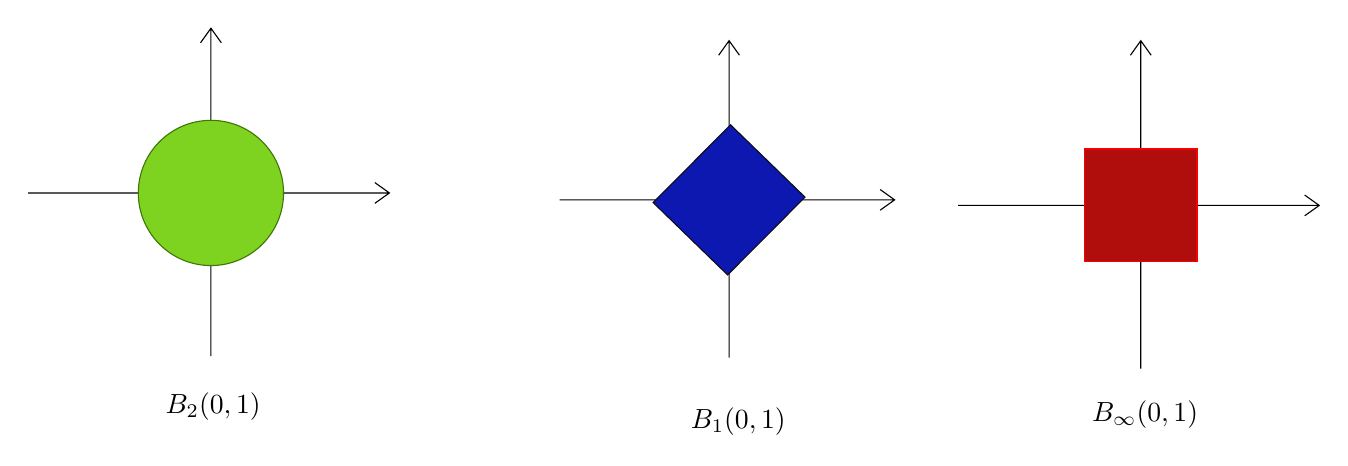
\begin{tikzpicture}[x=0.75pt,y=0.75pt,yscale=-1,xscale=1]
%uncomment if require: \path (0,300); %set diagram left start at 0, and has height of 300

%Shape: Axis 2D [id:dp5768057436819455] 
\draw  (466.67,160.37) -- (640.66,160.37)(554.7,81) -- (554.7,239) (633.66,155.37) -- (640.66,160.37) -- (633.66,165.37) (549.7,88) -- (554.7,81) -- (559.7,88)  ;
%Shape: Rectangle [id:dp28900760597735564] 
\draw  [color={rgb, 255:red, 249; green, 0; blue, 0 }  ,draw opacity=1 ][fill={rgb, 255:red, 176; green, 13; blue, 13 }  ,fill opacity=1 ] (527.59,133.18) -- (581.8,133.18) -- (581.8,187.56) -- (527.59,187.56) -- cycle ;
%Shape: Axis 2D [id:dp8071124205423666] 
\draw  (274.67,157.69) -- (436.09,157.69)(356.33,81) -- (356.33,233.67) (429.09,152.69) -- (436.09,157.69) -- (429.09,162.69) (351.33,88) -- (356.33,81) -- (361.33,88)  ;
%Shape: Rectangle [id:dp21020798758693604] 
\draw  [color={rgb, 255:red, 12; green, 12; blue, 30 }  ,draw opacity=1 ][fill={rgb, 255:red, 13; green, 24; blue, 176 }  ,fill opacity=1 ] (357.04,121.53) -- (392.91,156.38) -- (355.63,193.85) -- (319.76,159) -- cycle ;
%Shape: Axis 2D [id:dp5535257562468544] 
\draw  (18.67,154.37) -- (192.66,154.37)(106.7,75) -- (106.7,233) (185.66,149.37) -- (192.66,154.37) -- (185.66,159.37) (101.7,82) -- (106.7,75) -- (111.7,82)  ;
%Shape: Circle [id:dp5089540403949799] 
\draw  [color={rgb, 255:red, 65; green, 117; blue, 5 }  ,draw opacity=1 ][fill={rgb, 255:red, 126; green, 211; blue, 33 }  ,fill opacity=1 ] (71.71,154.37) .. controls (71.71,135.05) and (87.37,119.38) .. (106.7,119.38) .. controls (126.02,119.38) and (141.68,135.05) .. (141.68,154.37) .. controls (141.68,173.69) and (126.02,189.35) .. (106.7,189.35) .. controls (87.37,189.35) and (71.71,173.69) .. (71.71,154.37) -- cycle ;

% Text Node
\draw (529.99,253.24) node [anchor=north west][inner sep=0.75pt]    {$B_{\infty }( 0,1)$};
% Text Node
\draw (336.64,256.51) node [anchor=north west][inner sep=0.75pt]    {$B_{1}( 0,1)$};
% Text Node
\draw (83.64,249.4) node [anchor=north west][inner sep=0.75pt]    {$B_{2}( 0,1)$};


\end{tikzpicture}

\begin{definition}
 Soit $E$ un ensemble. Soient $x,y\in E$. Le segment liant $x$ et $y$ est l'ensemble
 \[
 \{tx+(1-t)y\mid t\in [0,1]\}
 \]
\end{definition}
\begin{definition}
    Soit $E$ un ensemble, $E$ est dit convexe si $\forall x,y\in E$, le segment liant $x$ et $y$ est inclus dans $E$.
\end{definition}
\begin{proposition}
    Soit $(E,\norm{\cdot})$ un EVN. Les boules ouvertes/fermées sont des ensembles convexes.
\end{proposition}
\begin{proof}
    Soit $B(a,r)$ une boule ouverte. $B(a,r)$ est convexe si et seulement si
    \[
    \forall x,y\in B(a,x), \forall t\in [0,1] \quad tx+(1-t)y\in B(a,r)
    \]
    Soient $x,y\in B(a,r)$ et $t\in [0,1]$ on a
    \[
    \norm{tx-(1-t)y-a}=\norm{tx-(1-t)y-ta+(1-t)a}\leq t\norm{x-a}+(1-t)\norm{y-a}<tr+(1-t)r=r
    \]
\end{proof}

On peut généralement parler d'ensembles ouverts et d'ensembles fermés

\begin{definition}
    Soit $(E,\norm{\cdot})$ un EVN.
    \begin{itemize}
        \item Un ensemble $A\subseteq E$ est ouvert si
        \[
        \forall a\in A, \exists r>0 \quad B(a,r)\subseteq A     \]
        \item Un ensemble $A$ est fermé si $E\setminus A$ est ouvert.
        \item Un point $a\in A$ est dit intérieur à l'ensemble $A$ si
        \[
        \exists r>0 \quad B(a,r)\subseteq A.
        \]
    \end{itemize}
\end{definition}
On remarque que $A$ est ouvert si $A$ coïncide avec son intérieur.
Les ouverts vérifient les propriétés suivantes
\begin{enumerate}
    \item $\varnothing$ et $E$ sont ouverts (et fermés)
    \item Une union quelconque d'ensembles ouverts est ouverte.
    \item Une intersection finie d'ensembles ouverts est ouverte.
\end{enumerate}
Il n'y a pas de contradiction avec les noms : boule ouverte/fermée.
\begin{proposition}
    Soit $(E,\norm{\cdot})$ un EVN. Toute boule ouverte est ouverte et toute boule fermée est fermée.
\end{proposition}
\begin{proof}
    Soit $B(a,r)$ une boule ouverte. Soit $x\in B(a,r)$, il faut montrer que $\exists\varepsilon >0 \quad B(x,\varepsilon)\subseteq B(a,r)$. Comme $x\in B(a,r)$, on a $\norm{x-a}<r$. Il existe donc $\varepsilon>0$ tel que $\norm{x-a}<r-\varepsilon$, soit $y\in B(x,\varepsilon)$ on a
    \[
    \norm{y-a}< \norm{y-x}+\norm{x-a}<\varepsilon+r-\varepsilon=r
    \]
    Soit $\overline{B(a,r)}$ une boule fermée. Soit $x\in E\setminus\overline{B(a,r)}$ on a $\norm{x-a}>r$ donc il existe $\varepsilon>0$ tel que $\norm{x-a}\geq r+\varepsilon$ montrons que $B(x,\varepsilon)\subseteq E\setminus\overline{B(a,r)}$, soit $y\in B(x,\varepsilon)$ on a
    \[
    \norm{y-x}\geq \norm{x-a}-\norm{y-x}>r+\varepsilon-\varepsilon=r
    \]
\end{proof}
La notion d'ensembles ouverts dépend fortement des boules qui elle même dépendent de la norme considérée.
\begin{definition}
    Soit $E$ un espace vectoriel. Deux normes sur $E$ sont dites équivalentes si elles induisent les mêmes ensembles ouverts. 
    
\end{definition}
\begin{remarque}
Il s'agit bien d'une relation d'équivalence, puisque l'égalité entre l'ensemble des ouverts en est une.
\end{remarque}
\begin{proposition}
    Soient $(E,\norm{\cdot})$ et $(E,\norm{\cdot}')$ des EVN. Les normes $\norm{\cdot}$ et $\norm{\cdot}'$ sont équivalentes s'il existe $C_1,C_2>0$ tel que
    \[
    \forall x\in E, C_1\norm{x}\leq \norm{x}'\leq  C_2\norm{x}
    \]
\end{proposition}
\begin{proof}
    $(\Leftarrow)$ Afin de montrer que les normes sont équivalentes et donc que la notion d'ouvert est la même pour ces deux normes, il suffit de montrer que pour tout $r>0$, il existe $\varepsilon,\varepsilon '>0$ tel que $B(a,\varepsilon)\subseteq B(a,r)$ et $B_(a,\varepsilon')\subseteq B(a,r)$. Soient $a\in E$ et $r>0$. Prenons $\varepsilon =\frac{r}{C_2}$ Soit $x\in B_{\norm{\cdot}}(a,\varepsilon)$ alors $\norm{x-a}'\leq C_2\norm{x-a}<C_2\varepsilon=r$ Soient $a\in E$ et $r>0$. Prenons $\varepsilon'=r\cdot C_1$
    Soit $x\in B_{\norm{\cdot}'}(a,\varepsilon')$. Alors $\norm{x-a}\leq \frac{1}{C_1}\norm{x-a}'<\frac{\varepsilon'}{C_1}=r$\\
    $(\Rightarrow)$ Par hypothèse, $B_{\norm{\cdot}}(0,1)$ est un ouvert pour la norme $\norm{\cdot}'$ et donc, il existe $r_1>0$ tel que$B_{\norm{\cdot}'}(0,r_1)\subseteq B_{\norm{\cdot}}(0,1)$? De même, il existe $r_2>0$ tel que$B_{\norm{\cdot}}(0,r_2)\subseteq B_{\norm{\cdot}'}(0,1)$ Soit $x\in E\setminus\{0\}$ On remarque $\frac{r_1x}{2\norm{x}}\in B_{\norm{\cdot}'}(0,r_1)$. On a donc $\frac{r_1}{2}\cdot\frac{x}{\norm{x}}\in B_{\norm{\cdot}}(0,1)$ i.e
    $\norm{\frac{r_1}{2}\cdot\frac{x}{\norm{x}}}<1$. On en déduit que $\frac{r_1}{2\norm{x}'}\norm{x}<1$ i.e $\frac{r_1}{2}\norm{x}<\norm{x'}$ En utilisant $B_{\norm{\cdot}}(0,r_2)\subseteq B_{\norm{\cdot}'}(0,1)$. On obtient l'existence d'un $C_2>0$ tel que $\norm{x}'\leq C_2\norm{x}$ pour tout $x\in E$
\end{proof}

\begin{remarque}[Exo]
    Soient $\norm{\cdot}$ et $\norm{\cdot}'$ deux normes équivalentes sur $E$.
    Une suite $(x_n)_{n\geq 1}\subseteq E$ converge vers $a\in E$ pour la norme $\norm{\cdot}$ si et seulement si elle converge vers $a$ pour la norme $\norm{\cdot}'$.
\end{remarque}

\begin{proposition}[Exo]
    Soient $E,F$ des espaces vectoriels
    \begin{itemize}
        \item $\norm{\cdot}_E,\norm{\cdot}'_E$ des normes équivalentes sur $E$
        \item $\norm{\cdot}_F,\norm{\cdot}'_F$ des norme équivalentes sur $F$
    \end{itemize}
    Une fonction $f:(E,\norm{\cdot}_E)\to (F,\norm{\cdot}_F) $ est continue en $a\in E$ ssi la fonction  $f:(E,\norm{\cdot}'_E)\to (F,\norm{\cdot}'_F) $ est continue en $a\in E$
\end{proposition}
\begin{theoreme}
    Sur un espace vectoriel $E$ de dimension finie, toutes les normes sont équivalentes.
\end{theoreme}
\begin{proof}
Pour montrer que les normes sont équivalentes, on va montrer qu'elles sont équivalentes à la norme $\norm{\cdot}_\infty$. 
Soit $\{e_1,...,e_n\}$ une base de $E$. Pour tout $x\in 
E$, on pose  $x:=\sum_{k=1}^nx_ke_k$. Soit $\norm{\cdot}$ une norme sur $E$. Soit $x\in E$. On a
    \[
    \norm{x}=\norm{\sum_{k=1}^nx_ke_k}\leq \sum_{k=1}^n|x_k|\norm{e_k}\leq\left(\sum_{k=1}^n\norm{e_k}\right)\norm{x}_{\infty}=:C_2\norm{x}_\infty
    \]
    Dans $(\mathbb{R}^n,\norm{\cdot}_\infty)$, la sphère unité $S=\{x\in \mathbb{R}^n\mid\norm{x}_\infty=1\}$ est compacte. La fonction $$\fonction{f}{(\mathbb{R}^n,\norm{\cdot}_\infty)\to (E,\norm{\cdot}_\infty)}{ (x_1, \dots, x_n) \mapsto \sum_{i = 1}^nx_ie_i}$$ est une isométrie linéaire (\textit{i.e.} un isomorphisme tel que $\forall x,\norm{x} = \norm{f(x)}$). $f$ est continue car $\norm{f(x)-f(a)}_\infty = \norm{f(x-a)}_\infty = \norm{x-a}_{\infty}$, il suffit de prendre $\delta = \varepsilon$.
    On en déduit que $f(S) = \{ x\in E \mid \norm{x}_\infty=  1\}$ est compact dans $E$. $\norm{\cdot} : (E,\norm{\cdots})\to \R^{\geq 0}$ est aussi continue, car $\exists C_2<0,\; \big|\norm x-\norm a \big|\leq\norm{x-a}\leq C_2\norm{x-a}_\infty$, et il suffit de prendre $\delta = \frac{\varepsilon}{C_2}$. Ainsi $\norm{\cdot}$ sur $\{ x\in E \;|\; \norm{x}_\infty=  1\}$ atteint ses bornes, en particulier son minimum.
    Donc il existe $z\in E,\; \norm z _\infty = 1$ et $\forall x  \in E$ tel que $\norm{x}_\infty = 1$, on a $\norm x \geq \norm z $. Soit $x\in E\setminus \{0\}$. Considérons $\dfrac{x}{\norm x _\infty}$. Comme sa $\infty$-norme vaut $1$, on en conclut que $\norm{\dfrac{x}{\norm x _\infty}}\geq \norm z $ d'où, en posant $C_1 = \norm{z}$, $\norm x \geq C_1\norm x _\infty$
\end{proof}
\begin{exemple}
    Montrons que les normes ne sont pas nécessairement équivalentes en dimension infinie. Pour ce faire, considérons le $\R$-espace vectoriel $X:=\{f:[0,\;1]\to\R $ application continue $\}$. On définit deux normes sur $X$ : $\norm{f}_\infty = \max_{x\in [0,\;1]}|f(x)|$ et $\norm{f}_1 = \int_0^1|f(x)|dx$. Pour tout $n\in\N$ posons $f_n(x) := x^n$. Remarquons que $\norm{f_n}_\infty = 1$, alors que $\norm{f_n}_1 = \int_0^1x^ndx = \dfrac 1 {n+1} \to 0$ quand $n\to +\infty$. Ainsi, il n'existe pas de constante $C>0$ telle que $\forall f\in X, \norm f_\infty\leq C\cdot\norm f _1$, donc $\norm\cdot_\infty et \norm\cdot _1$ ne sont pas équivalentes.
\end{exemple}
\begin{notation}
    Soient $(E,\norm\cdot_E),(F,\norm \cdot_F)$ deux EVN.
    On note $L(E,F):=\{f:E\to F\mid f$ est linéaire$\}$
\end{notation}
\begin{proposition}
    Soient $(E,\norm\cdot_E),(F,\norm \cdot_F)$ deux EVN. Si $E$ est de dimension finie, alors toute application dans $L(E,F)$ est continue.
\end{proposition}
\begin{proof}
    Soit $f\in L(E,F)$.
    Par équivalence des normes, il suffit de montrer que $f$ est continue de $(E,\norm\cdot _1)$ dans $(F,\norm \cdot_F)$. Soit $(e_1,\dots,e_n)$ une base de $E$. Soit $\varepsilon>0$. Posons $\alpha := \max_{1\leq k \leq n}\norm{f(e_k)}_F$. Prenons $\delta = \frac \varepsilon {\alpha+1}$.
    Soit $x\in E$ tel que $\norm{x-a}_1\leq \delta$. On a alors
    \begin{align*}
    \norm{f(x)-f(a)}_F & =\norm{f(x-a)}_F := \norm{f\left(\sum_{k=1}^n(x_k-a_k)e_k\right)}_F\\
    &=\norm{\sum_{k=1}^n(x_k-a_k)f(e_k)}_F\\
    &\leq \sum_{k=1}^n|x_k-a_k|\norm{f(e_k)}_F\leq \sum_{k=1}^n|x_k-a_k|\alpha\\
    &=\alpha\norm{x-a}_1\leq\varepsilon
    \end{align*}
\end{proof}

Sur $\R^n$, on pourra donc travailler avec la norme que l'on souhaite, car elles sont toutes équivalentes. Cependant, dans le cadre des espaces vectoriels de dimension infinie, il faudra faire attention à la norme que l'on choisit.
On va maintenant montrer que toute application linéaire sur un espace vectoriel normé de dimension finie est continue.

\begin{notation}
    Si $E$ est de dimension finie, on peut munir $L(E,F)$ d'une norme :$$\norm f_{L(E,F)} = \sup_{x\in B_E(0,1)}\norm {f(x)}_F$$
\end{notation}
En effet, on a $\norm{f(x)}_F = \norm{f\left(\norm{x}_E\frac{x}{\norm{x}_E}\right)}_F = \norm{x}_E\norm{f\left(\frac{x}{\norm{x}_E}\right)}_F\leq \norm{x}_E\norm f_{L(E,F)}$.

\section{\texorpdfstring{$*$ $p$-norme $*$}{* p-norme *}}
Soit $p\in[1,+\infty[$. On peut définir une norme sur $\R ^n$ par $\norm\cdot_p = \left(\sum_{i=1}^n|x_i|^p\right)^{\frac 1 p}$.
\begin{proposition}
    Pour tout $p\in[0,+\infty[,\norm{\cdot}_p$ est une norme
    \begin{proof}
        Seule l'inégalité triangulaire n'est pas triviale, et elle est appelée inégalité de Minkowski.
        %En chantier
    \end{proof}
\end{proposition}
\begin{proposition}
    Soit $x\in\R^n$. On supposera $p\in[1,+\infty[ $ dans la suite de la preuve. On a $\lim_{p\to+\infty}\norm{x}_p=\norm x _\infty$.
\end{proposition}
    \begin{proof}
        Rappelons que $\norm x_\infty:=\max_{1\leq i\leq n}\abs{x_i}$. Il vient donc
        \begin{align*}
            \norm{x}_\infty &= (\norm{x}_\infty ^p)^{\frac 1 p}\leq\left(\sum_{i=1}^n|x_i|^p\right)^{\frac 1 p}\\
            &\leq\left(\sum_{i=1}^n\norm{x}_\infty^p\right)^{\frac 1 p}=n^{\frac 1 p}\cdot\norm{x}_\infty
        \end{align*}
        Par le théorème du sandwich, le résultat suit.
    \end{proof}

    